\begin{corrige}{devoir2-0007}
  \begin{enumerate}
  \item 
    \begin{enumerate}
    \item[(a)] La région à décrire ressemble à un quart d'œuf. En coordonnées cylindriques $\theta\in [-\pi/2, 0]$ à cause des inégalités $x>0$ et $y<0$ et $z\in [-\sqrt{9-r^2}, 9-r^2]$. L'intersection entre la  boule de rayon $3$ centrée en l'origine et le paraboloïde elliptique $z=9-r^2$ est le disque de  rayon $3$, centre $(0,0,0)$ sur le plan $x$-$y$. Dans la figure, il faut faire attention parce que les échelles des deux axes ne sont pas les mêmes. 

      Les équations en coordonnées sphériques sont $\theta\in [-\pi/2, 0]$, $\rho\cos(\phi)\leq 9- \rho^2\sin^2(\phi)$, pour $\phi$ dans l'intervalle $[0, \pi/2]$ et $\rho\leq 3$ pour  $\phi$ dans l'intervalle $[\pi/2, \pi]$.
 \begin{figure}
  \begin{center}
    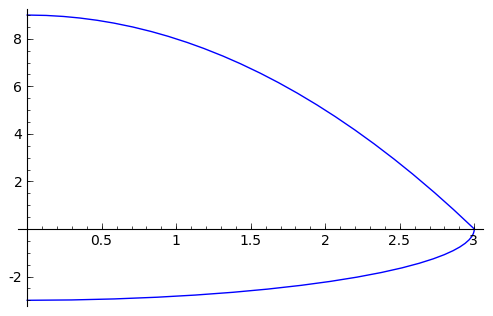
\includegraphics[width=7cm]{Fig_exo6devoir2premiere.png}
    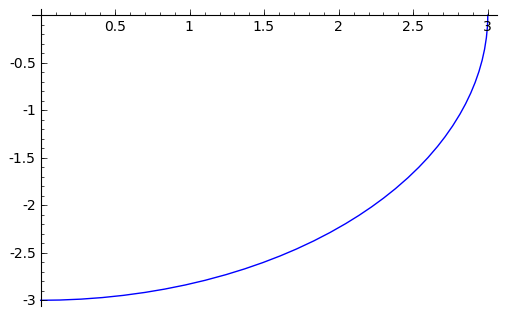
\includegraphics[width=7cm]{Fig_exo6devoir2premiere_a.png} 

  \caption{Les projections sur le plans $z$-$x$ et $x$-$y$ de la région décrite dans l'exercice 6.1.(a)}\label{exo6devoir2}
  \end{center}
 
  \end{figure}
    \item[(b)] Il suffit de multiplier l'équation par $\rho$ pour comprendre que il s'agit de l'équation du plan $x+z=0$. En coordonnées cylindriques on peut l'écrire comme $r\cos(\theta)+z=0$. 
    \end{enumerate}

\begin{figure}
  \begin{center}
     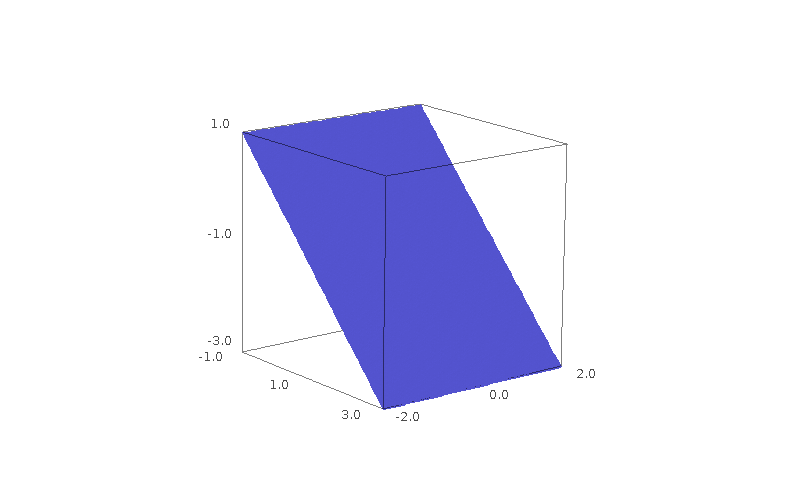
\includegraphics[width=7cm]{Fig_exo6devoir2deuxieme.png}

  \caption{La surface décrite dans l'exercice 6.1.(b)}\label{exo6devoir2un}
  \end{center}
 
  \end{figure}

  \item Les inéquations en coordonnées cylindriques sont 
    \begin{equation}
      \begin{cases}
        -1\leq z\leq 1,\\
        \sqrt{1-z^2}\leq\sqrt{x^2+y^2},\\
        \sqrt{x^2+y^2}\leq 1.
      \end{cases}
    \end{equation}
    On peut enlever les racines carrées dans la deuxième et la troisième. On voit alors que la région à décrire est bornée entre la boule de centre $(0,0,0)$ et rayon  $1$ et le cylindre de base $x^2+y^2\leq 1$, symétrique par rapport à l'axe des $z$ centré en l'origine et de hauteur totale $2$.  
  \end{enumerate}

\begin{figure}
  \begin{center}
    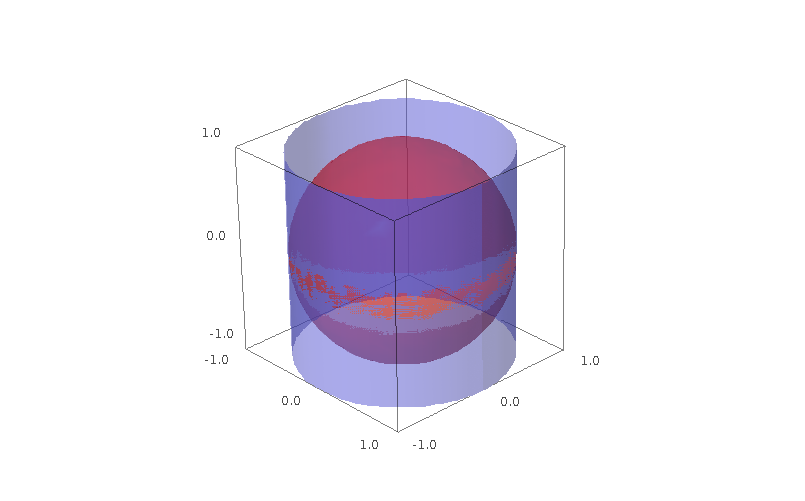
\includegraphics[width=7cm]{Fig_exo6devoir2troisieme.png}

  \caption{La région décrite dans la deuxième partie de l'exercice 6}\label{exo6devoir2deux}
  \end{center}
 
  \end{figure}

\end{corrige}
